% Fonte das figuras das distâncias declaradas (Figura 2.1 do TG).
% Compilar com: pdflatex fig_distancias_declaradas.tex
% Gera um PDF de duas páginas: (1) esquema da pista; (2) fluxograma de dependência.
% Copiar o resultado para Figures/fig_distancias_declaradas.pdf.
\documentclass[12pt, tikz, border=2pt]{standalone}
\usepackage[utf8]{inputenc}
\usepackage[T1]{fontenc}
\usepackage{mathptmx}
\usetikzlibrary{arrows.meta, positioning, patterns, calc}
\begin{document}
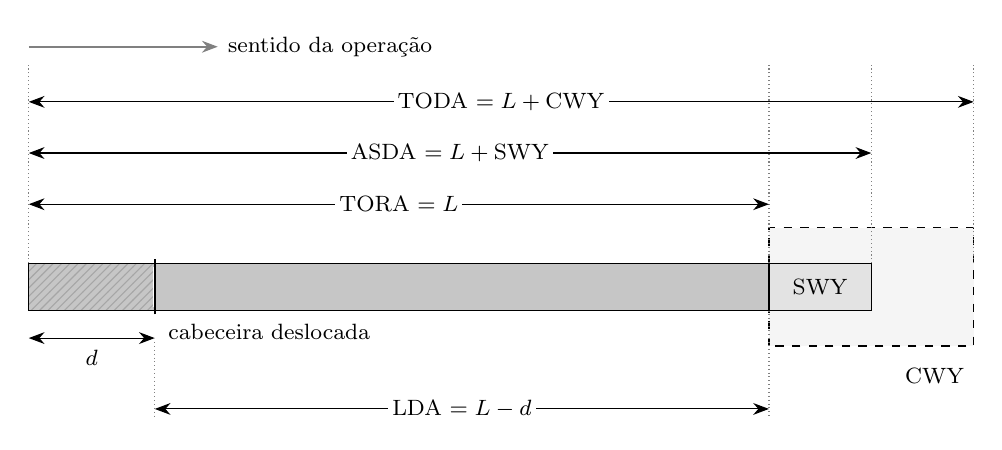
\begin{tikzpicture}[
    >={Stealth[length=2mm]},
    cota/.style={<->, thin},
    guia/.style={densely dotted, thin, gray},
    rotulo/.style={font=\footnotesize, fill=white, inner sep=1.5pt},
]
    % geometria (1 unidade = 1 cm; fora de escala)
    \def\L{9.4}\def\d{1.6}\def\swy{1.3}\def\cwy{2.6}
    % zona livre de obstáculos (fundo)
    \draw[dashed, fill=gray!8] (\L,-0.45) rectangle (\L+\cwy,1.05);
    \node[font=\footnotesize, anchor=south east] at (\L+\cwy,-1.05) {CWY};
    % pista e zona de parada
    \fill[gray!45] (0,0) rectangle (\L,0.6);
    \fill[pattern=north east lines, pattern color=gray!70] (0,0) rectangle (\d,0.6);
    \draw (0,0) rectangle (\L,0.6);
    \draw[fill=gray!22] (\L,0) rectangle (\L+\swy,0.6);
    \node[font=\footnotesize] at (\L+\swy/2,0.3) {SWY};
    % cabeceira deslocada
    \draw[very thick, white] (\d,0.05) -- (\d,0.55);
    \draw[thick] (\d,-0.05) -- (\d,0.65);
    \node[font=\footnotesize, anchor=north west] at (\d+0.05,-0.05) {cabeceira deslocada};
    \draw[cota] (0,-0.35) -- (\d,-0.35);
    \node[font=\footnotesize, anchor=north] at (\d/2,-0.38) {$d$};
    % sentido da operação
    \draw[->, thick, gray] (0,3.35) -- (2.4,3.35)
        node[right, font=\footnotesize, text=black] {sentido da operação};
    % linhas de chamada
    \foreach \x in {0, \L, \L+\swy, \L+\cwy} \draw[guia] (\x,0.6) -- (\x,3.15);
    \draw[guia] (\d,-0.4) -- (\d,-1.35);
    \draw[guia] (\L,0) -- (\L,-1.35);
    % cotas
    \draw[cota] (0,1.35) -- node[rotulo] {TORA $= L$} (\L,1.35);
    \draw[cota] (0,2.0) -- node[rotulo] {ASDA $= L + \mathrm{SWY}$} (\L+\swy,2.0);
    \draw[cota] (0,2.65) -- node[rotulo] {TODA $= L + \mathrm{CWY}$} (\L+\cwy,2.65);
    \draw[cota] (\d,-1.25) -- node[rotulo] {LDA $= L - d$} (\L,-1.25);
\end{tikzpicture}

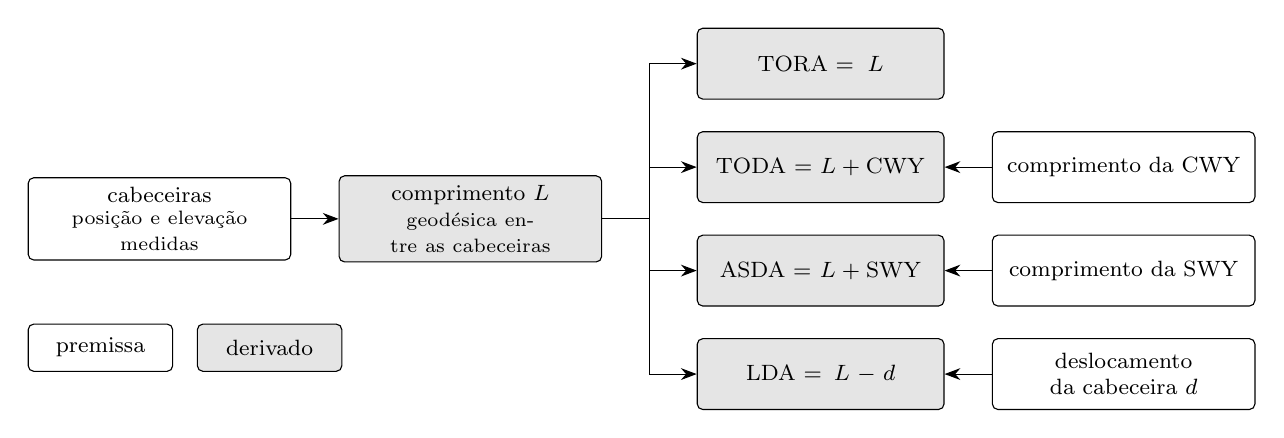
\begin{tikzpicture}[
    >={Stealth[length=2mm]},
    node distance=4mm and 6mm,
    premissa/.style={draw, rounded corners=2pt, align=center, font=\footnotesize,
                     minimum height=9mm, text width=31mm},
    derivado/.style={premissa, fill=gray!20},
    distancia/.style={derivado, text width=29mm},
]
    % coluna central: distâncias declaradas
    \node[distancia] (tora) {TORA $= L$};
    \node[distancia, below=of tora] (toda) {TODA $= L + \mathrm{CWY}$};
    \node[distancia, below=of toda] (asda) {ASDA $= L + \mathrm{SWY}$};
    \node[distancia, below=of asda] (lda)  {LDA $= L - d$};
    % barramento do comprimento
    \coordinate (bus) at ($(tora.west)!0.5!(lda.west) + (-6mm,0)$);
    \node[derivado, left=6mm of bus] (L) {comprimento $L$\\ \scriptsize geodésica entre as cabeceiras};
    \node[premissa, left=of L] (cab) {cabeceiras\\ \scriptsize posição e elevação\\ \scriptsize medidas};
    \draw[->] (cab) -- (L);
    \draw (L.east) -- (bus);
    \draw (bus |- tora.west) -- (bus |- lda.west);
    \foreach \n in {tora, toda, asda, lda} \draw[->] (bus |- \n.west) -- (\n.west);
    % premissas próprias de cada distância
    \node[premissa, right=of toda] (cwy) {comprimento da CWY};
    \node[premissa, right=of asda] (swy) {comprimento da SWY};
    \node[premissa, right=of lda]  (dd)  {deslocamento da cabeceira $d$};
    \draw[->] (cwy) -- (toda);
    \draw[->] (swy) -- (asda);
    \draw[->] (dd)  -- (lda);
    % legenda
    \node[premissa, text width=16mm, minimum height=6mm, below=8mm of cab.south west, anchor=north west]
        (lp) {premissa};
    \node[derivado, text width=16mm, minimum height=6mm, right=3mm of lp] {derivado};
\end{tikzpicture}
\end{document}
